\documentclass[tikz,border=0.1in]{standalone}
\usepackage{tikz}
\usetikzlibrary{positioning, arrows.meta, fit, backgrounds, calc}
\usepackage[T1]{fontenc}
\usepackage{amssymb}
\usepackage[scaled=0.95]{helvet}
\renewcommand{\familydefault}{\sfdefault}

\definecolor{miamired}{HTML}{C3142D}
\definecolor{agentblue}{HTML}{1D5FAD}
\definecolor{evalgold}{HTML}{EFDB72}
\definecolor{nonfund}{HTML}{CCC9B8}

\tikzset{
  entry/.style  = {rectangle, rounded corners, draw=gray!70, ultra thick,
                   fill=gray!6, align=center, text width=3.1cm, minimum height=1.6cm,
                   font=\small\bfseries, inner sep=5pt},
  route/.style  = {rectangle, rounded corners, draw=agentblue, ultra thick,
                   fill=agentblue!6, align=center, text width=3.6cm, minimum height=1.6cm,
                   font=\small, inner sep=5pt},
  cached/.style = {rectangle, rounded corners, draw=miamired, ultra thick,
                   fill=miamired!8, align=center, text width=5.9cm, minimum height=1.6cm,
                   font=\small, inner sep=5pt},
  live/.style   = {rectangle, rounded corners, draw=agentblue, ultra thick, dashed,
                   fill=agentblue!4, align=center, text width=5.9cm, minimum height=1.6cm,
                   font=\small, inner sep=5pt},
  lab/.style    = {font=\small, align=center},
  flow/.style   = {ultra thick, -{Stealth[length=3mm]}, draw=miamired!65},
}

\begin{document}
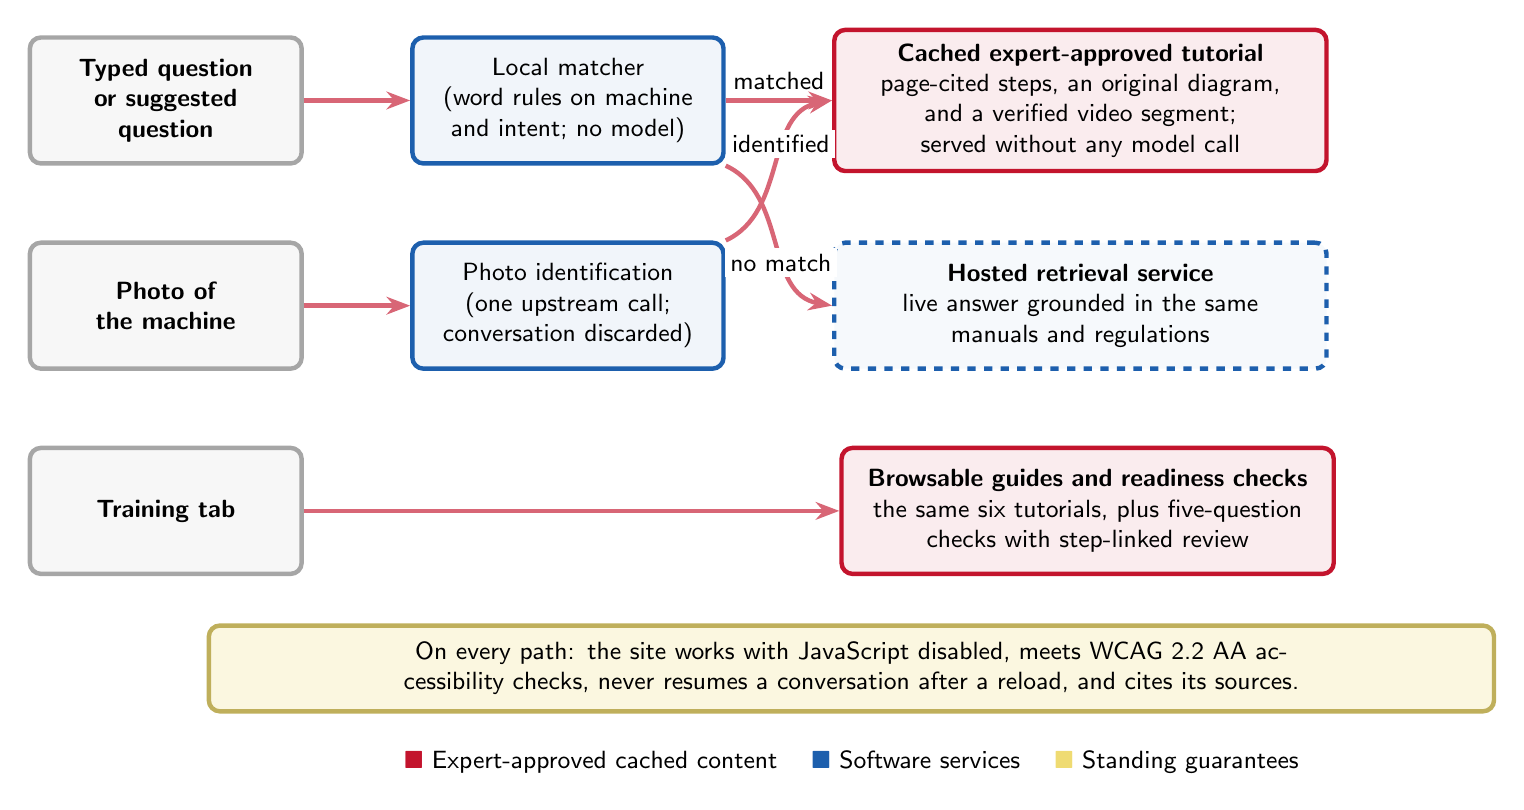
\begin{tikzpicture}[node distance=0.95cm and 1.35cm]

% Entry column
\node (e1) [entry]              {Typed question\\or suggested\\question};
\node (e2) [entry, below=of e1] {Photo of\\the machine};
\node (e3) [entry, below=of e2] {Training tab};

% Routing column
\node (m1) [route, right=of e1] {Local matcher\\(word rules on machine\\and intent; no model)};
\node (m2) [route, right=of e2] {Photo identification\\(one upstream call;\\conversation discarded)};

% Outcome column
\node (o1) [cached, right=of m1] {\textbf{Cached expert-approved tutorial}\\page-cited steps, an original diagram,\\and a verified video segment;\\served without any model call};
\node (o2) [live, right=of m2]  {\textbf{Hosted retrieval service}\\live answer grounded in the same\\manuals and regulations};
\node (o3) [cached, right=of e3, xshift=5.45cm] {\textbf{Browsable guides and readiness checks}\\the same six tutorials, plus five-question\\checks with step-linked review};

% Flows
\draw [flow] (e1) -- (m1);
\draw [flow] (m1) -- node[lab, above] {matched} (o1);
\draw [flow] (m1.south east) to[out=-25,in=170] (o2.west);
\draw [flow] (e2) -- (m2);
\draw [flow] (m2.north east) to[out=25,in=190] (o1.west);
% Branch labels anchored just outside each destination, clear of the crossing
\node [lab, fill=white, inner sep=2pt] at ($(o1.west)+(-0.65,-0.55)$) {identified};
\node [lab, fill=white, inner sep=2pt] at ($(o2.west)+(-0.65,0.55)$) {no match};
\draw [flow] (e3) -- (o3);

% Guarantees band
\node (band) [lab, below=0.6cm of o3.south, xshift=-3.0cm, text width=15.9cm,
  draw=evalgold!80!black, ultra thick, fill=evalgold!22, rounded corners,
  inner sep=6pt] {%
  On every path: the site works with JavaScript disabled, meets WCAG 2.2 AA
  accessibility checks, never resumes a conversation after a reload, and cites
  its sources.};

% Legend
\node [font=\small, anchor=north] at ($(band.south)+(0,-0.35)$) {%
  \textcolor{miamired}{$\blacksquare$}~Expert-approved cached content \quad
  \textcolor{agentblue}{$\blacksquare$}~Software services \quad
  {\color{evalgold}$\blacksquare$}~Standing guarantees};

\end{tikzpicture}
\end{document}
